%%%%%%%%%%%%%%%%%%%%%%%%%%%%%%%% COMMENT THIS TO COMPILE main.tex %%%%%%%%%%%%%%%%%%%%%%%%%%%%%%%%
\documentclass[a4paper,12pt]{report}
\usepackage[english]{babel}
\usepackage[left=2cm,right=2cm,top=2cm,bottom=2cm]{geometry}
%\usepackage{mathtools}
\usepackage{amsthm}     % for definitions and theorems
\usepackage[many]{tcolorbox}    % boxes around definitions and theorems
%\usepackage{amsmath}
%\usepackage{nccmath}
\usepackage{amssymb}    % \ltimes
\usepackage{etoolbox}   % for start of Chapter
%\usepackage{amsfonts}
\usepackage{physics}    % for all Physics related
\usepackage{dsfont}     % for the identity matrix symbol \1
%\usepackage{mathrsfs}

\usepackage{titling}
\usepackage{indentfirst}

\usepackage{bm}
\usepackage[dvipsnames]{xcolor}
\usepackage{cancel}

\usepackage{xurl}
\usepackage[colorlinks=true]{hyperref}

\usepackage{float}
\usepackage{graphicx}
\usepackage{subcaption}
%\usepackage{tikz}

\usepackage{ctable}     % tabelas
\renewcommand{\P}{\phantom{+}}  % empty space to indent things
\usepackage{multirow}
\usepackage{tabulary}

%%%%%%%%%%%%%%%%%%%%%%%%%%%%%%%%%%%%%%%%%%%%%%%%%%%

\newcommand{\eps}{\epsilon}
\newcommand{\vphi}{\varphi}
\newcommand{\cte}{\text{cte}}

\newcommand{\N}{{\mathbb{N}}}
\newcommand{\Z}{{\mathbb{Z}}}
%\newcommand{\Q}{{\mathbb{Q}}}
\newcommand{\C}{{\mathbb{C}}}
\renewcommand{\S}{{\hat{S}}}
%\renewcommand{\H}{\s{H}}

\renewcommand{\a}{{\vb{a}}}
\renewcommand{\b}{{\vb{b}}}
\renewcommand{\d}{{\dagger}}
\newcommand{\up}{{\uparrow}}
\newcommand{\down}{{\downarrow}}
\newcommand{\hc}{{\text{h.c.}}}

\newcommand{\ihat}{\bm{\hat{\imath}}}
\newcommand{\jhat}{\bm{\hat{\jmath}}}
\newcommand{\khat}{\bm{\hat{k}}}

\newcommand{\0}{{\vb{0}}}
\newcommand{\1}{\mathds{1}}
\newcommand{\E}{{\vb{E}}}
\newcommand{\B}{{\vb{B}}}
\renewcommand{\u}{{\vb{u}}}
\renewcommand{\v}{{\vb{v}}}
\renewcommand{\r}{{\vb{r}}}
\newcommand{\R}{{\vb{R}}}
\newcommand{\Q}{{\vb{Q}}}
\newcommand{\G}{{\vb{G}}}
\newcommand{\g}{{\vb{g}}}
\renewcommand{\k}{{\vb{k}}}
\newcommand{\K}{{\vb{K}}}
\newcommand{\p}{{\vb{p}}}
\newcommand{\q}{{\vb{q}}}
\newcommand{\F}{{\vb{F}}}
\renewcommand{\t}{{\vb{t}}}
\newcommand{\vtau}{{\bm{\tau}}}
\newcommand{\vdelta}{{\bm{\delta}}}

% COLORED SYMMETRY ELEMENTS
\newcommand{\Ct}{{\textcolor{Cyan}{C_3}}}
\newcommand{\Ctn}[1]{{\textcolor{Cyan}{C_3^{\textcolor{black}{#1}}}}}
\newcommand{\Cs}{{\textcolor{ForestGreen}{C_6}}}
\newcommand{\Csn}[1]{{\textcolor{ForestGreen}{C_6^{\textcolor{black}{#1}}}}}
\newcommand{\sd}{{\textcolor{RoyalBlue}{\sigma_d}}}
\newcommand{\sdn}[1]{{\textcolor{RoyalBlue}{\sigma_d^{\textcolor{black}{#1}}}}}
\newcommand{\sdp}{{\textcolor{RoyalBlue}{\sigma_d'}}}
\newcommand{\sdpp}{{\textcolor{RoyalBlue}{\sigma_d''}}}
\newcommand{\sv}{{\textcolor{Orange}{\sigma_v}}}
\newcommand{\svn}[1]{{\textcolor{Orange}{\sigma_v^{\textcolor{black}{#1}}}}}
\newcommand{\svp}{{\textcolor{Orange}{\sigma_v'}}}
\newcommand{\svpp}{{\textcolor{Orange}{\sigma_v''}}}

\newcommand{\s}{\sigma}
%\newcommand{\prodint}[2]{\left\langle #1 , #2 \right\rangle}
\newcommand{\cc}[1]{\overline{#1}}
\newcommand{\Eval}[3]{\eval{\left( #1 \right)}_{#2}^{#3}}
\newcommand{\sg}[2]{\{ #1 \mid #2 \}}

\newcommand{\unit}[1]{\; \mathrm{#1}}

\newcommand{\n}{\medskip}
\newcommand{\e}{\quad \mathrm{and} \quad}
\newcommand{\ou}{\quad \mathrm{or} \quad}
\newcommand{\virg}{\, , \;}
\newcommand{\ptodo}{\forall \,}
\renewcommand{\implies}{\; \Rightarrow \;}
%\newcommand{\eqname}[1]{\tag*{#1}} % Tag equation with name

\setlength{\droptitle}{-7em}

\makeatletter
\patchcmd{\chapter}{\if@openright\cleardoublepage\else\clearpage\fi}{}{}{}  % start 'Chapter' at the same page. needs package etoolbox
\makeatother

%% Theorems, definitions, proofs
\theoremstyle{definition}

\newtheorem{definition}{Definition}[section]
\tcolorboxenvironment{definition}{
  colback=blue!5!white,
  boxrule=0pt,
  boxsep=1pt,
  left=2pt,right=2pt,top=2pt,bottom=2pt,
  oversize=2pt,
  sharp corners,
  before skip=\topsep,
  after skip=\topsep,
}

\newtheorem{theorem}{Theorem}[section]
\tcolorboxenvironment{theorem}{
  colback=blue!5!white,
  boxrule=0pt,
  boxsep=1pt,
  left=2pt,right=2pt,top=2pt,bottom=2pt,
  oversize=2pt,
  sharp corners,
  before skip=\topsep,
  after skip=\topsep,
}

\begin{document}
%%%%%%%%%%%%%%%%%%%%%%%%%%%%%%%% COMMENT THIS TO COMPILE main.tex %%%%%%%%%%%%%%%%%%%%%%%%%%%%%%%%


%%%%%%%%%%%%%%%%%%%%%%%%%%%%%%%%%%%%%%%%%%%%%%%%%%%%%%%%%%%%%%%%%%%%%%%%%%%%%%%%%%%%%%%%%%%%%%%%%%
\chapter{Sei lá}
%%%%%%%%%%%%%%%%%%%%%%%%%%%%%%%%%%%%%%%%%%%%%%%%%%%%%%%%%%%%%%%%%%%%%%%%%%%%%%%%%%%%%%%%%%%%%%%%%%

The concept of \textit{symmetry} reincidentally appears in physics, because various aspects of our reality exhibit symmetric objects.

Our goal is to develop a fully symmetric model for TBG. To achieve this, it is essential to first understand the mathematical concepts of symmetry, specifically Group Theory and Representation Theory as applied to crystallographic solids. In this chapter we will provide the necessary definitions and theorems in order to develop our symmetry analysis.

%%%%%%%%%%%%%%%%%%%%%%%%%%%%%%%%%%%%%%%%%%%%%%%%%%%%%%%%%%%%%%%%%%%%%%%%%%%%%%%%%%%%%%%%%%%%%%%%%%
\section{Elements of Group Theory}
%%%%%%%%%%%%%%%%%%%%%%%%%%%%%%%%%%%%%%%%%%%%%%%%%%%%%%%%%%%%%%%%%%%%%%%%%%%%%%%%%%%%%%%%%%%%%%%%%%

%%%%%%%%%%%%%%%%%%%%%%%%%%%%%%%%%%%%%%%%%%%%%%%%%%%%%%%%%%%%%%%%%%%%%%%%%%%%%%%%%%%%%%%%%%%%%%%%%%
%\subsection{Groups, cosets, and conjugacy classes}
%%%%%%%%%%%%%%%%%%%%%%%%%%%%%%%%%%%%%%%%%%%%%%%%%%%%%%%%%%%%%%%%%%%%%%%%%%%%%%%%%%%%%%%%%%%%%%%%%%

In this thesis we are concerned with symmetries that relate to graphene. Because its carbon atoms form a honeycomb lattice, our basic object of study will be a 2D hexagon.

\begin{figure}[H]
\centering
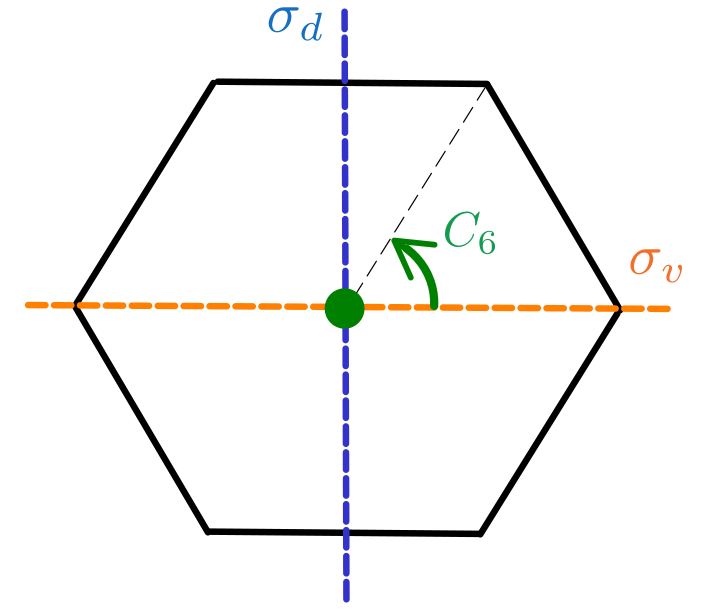
\includegraphics[width=0.4\linewidth]{fig/hexagon.png}
\caption{2D spatial symmetries of a hexagon.}
\label{fig:hexagon}
\end{figure}

In a certain sense, a basic hexagon has 12 symmetry elements. Looking at Figure \ref{fig:hexagon}, the hexagon has the reflections $\sd$, $\sv$, the $60^\circ$ rotation $\Cs$, and all the combinations of these. Combining all the possibilities, we say all that the symmetry elements of the hexagon form the \textit{group}
$$
D_6 = \{E, \Cs, \underbrace{\Ct}_{\Csn{2}}, \underbrace{C_2}_{\Csn{3}}, \underbrace{\Ctn{2}}_{\Csn{4}}, \Csn{5}, \sd, \underbrace{\sdp}_{\sdp \Ct}, \underbrace{\sdpp}_{\sdp \Ctn{2}}, \sv, \underbrace{\svp}_{\svp \Ct}, \underbrace{\svpp}_{\svp \Ctn{2}} \}.
$$
In this list, we did not include repeated elements, observe that $\Csn{6} = \sdn{2} = \svn{2} = E$ is the element the identity element, the one that ``does nothing''.

\n

The concept of \textit{group} $G$ grasps the set of elements $a \in G$ that represent the symmetry of an object, along with its symmetry operation ``$\vdot$''. The element $a \vdot b$ represents the ``composition'' of applying first the operation $a$, and then $b$.

\begin{definition}[\textbf{Group}]
Given a set $G$ and a binary operation ``$\vdot$''$:G\times G \to G$, \textbf{the pair} $(G, \vdot)$ is called a \textit{group} if it satisfies the following properties:
\begin{enumerate}
\item (closure): $a \vdot b \in G$, for every $a, b \in G$.
\item (associativity): $(a \vdot b) \vdot c =  a \vdot (b \vdot c)$, for every $a, b, c \in G$.
\item (identity): There exists an (identity) element $E \in G$ such that $E \vdot a = a \vdot E = a$, for every $a \in G$.
\item (inverse): For every $a \in G$, there is (an inverse) $a^{-1} \in G$ such that $a \vdot a^{-1} = a^{-1} \vdot a = E$.
\end{enumerate}
\end{definition}
Normally in the literature, one speaks of the set $G$ as being ``the group'' instead of the pair $(G, \vdot)$ and omits the operation symbol ``$\vdot$'', simply writing $ab$ instead of $a \vdot b$. This is for convenience but, mathematically, the operation ``$\vdot$'' is crucial to define a group.

\begin{definition}[\textbf{Order}]
The order of a group $G$ is defined as its number of elements $\abs{G}$.
\end{definition}

It happens frequently that an object $A$ has all the symmetries of another object $B$. For example, a hexagon has all the symmetries of a triangle, as we can see in Figure \ref{fig:hexagon_subgroup}.
\begin{figure}[H]
\centering
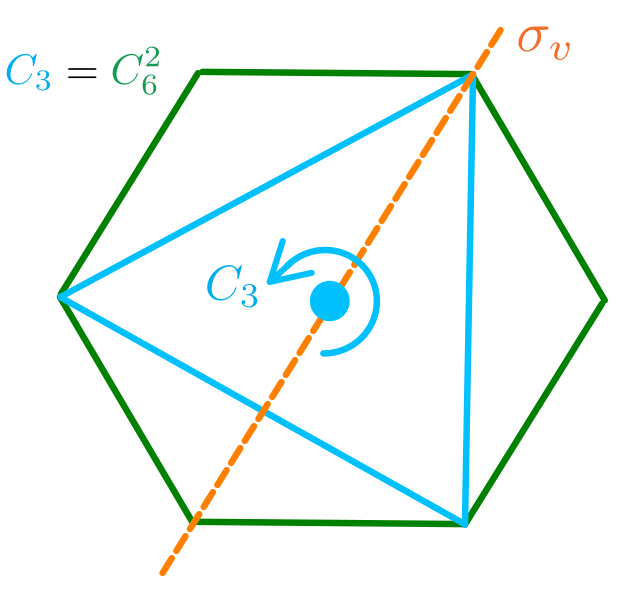
\includegraphics[width=0.4\linewidth]{fig/hexagon_subgroup.png}
\caption{The \textcolor{ForestGreen}{hexagon} has all the symmetries of the \textcolor{Cyan}{triangle}, i.e., $D_3$ is a subgroup of $D_6$.}
\label{fig:hexagon_subgroup}
\end{figure}

The symmetry elements of the triangle form the group $D_3 = \{E, \Ct, \Ctn{2}, \sv, \svp, \svpp\}$. Because $D_3$ is a subset of $D_6$ and also forms a group by itself, we say that $D_3$ is a subgroup of $D_6$.


\begin{definition}[\textbf{Subgroup}]
If $(G, \vdot)$ is a group and $H$ is a subset of $G$, we say that $H$ is a subgroup of $G$ if the pair $(H, \vdot)$ is a group by itself.
\end{definition}

It is common that one defines a group by its \textit{generators}. We did that when defining the groups $D_6$ and $D_3$ associated to the hexagon and triangle, respectively at Figures \ref{fig:hexagon} and \ref{fig:hexagon_subgroup}. By generators, we mean:

\begin{definition}[\textbf{Generators of a group}]
If $S$ is a subset of a group $G$, we define $\ev{S}$ as the smallest subgroup of $G$ containing every element of $S$. The subgroup $\ev{S}$ is called the \textit{subgroup generated by $S$}. If $\ev{S} = G$, we say that the set $S$ \textit{generates} $G$.
\end{definition}

An intuitive way of thinking of $\ev{S}$ is by ``recursively multiplying'' all the elements of $S$, until all the possibilities are exhausted. For example, in general for two elements:
$$
\ev{\{a,b\}} = \{E, a, b, a^2, ab, ba, b^2, a^3, a^2b, aba, ba^2, ab^2, bab, b^2a, b^3, \ldots\}.
$$

For the hexagon at Figure \ref{fig:hexagon}, the set $\{\Cs, \sd, \sv\}$ generates the group $D_6$; and for the triangle at Figure \ref{fig:hexagon_subgroup}, the set $\{\Ct, \sv\}$ generates the group $D_3$.

\begin{definition}[\textbf{Cosets}]
Let $G$ be a group and $H$ one of its subgroups. Given an element $g \in G$, we define the set $gH$ by
$$
gH = \{g h \mid h \in H\} \subseteq G.
$$
This set $gH$ is called a left coset of $G$ with respect to $H$, and $g$ is a representative of $gH$.

It is always possible to decompose $G$ as a disjoint union of its left cosets:
$$
G = \sum_{j=1}^{\abs{G:H}} g_j H,
$$
where $g_j \in G$ is a representative of $g_j H$, and $\abs{G:H}$ is the number of different left cosets.
\end{definition}

An iconic theorem due to Laplace says that the order of a subgroup $H \subseteq G$ divides the order of the group $G$.

\begin{theorem}[\textbf{Laplace}]
The number of different left cosets is given by $\abs{G:H} = \abs{G} / \abs{H}$.
\end{theorem}

As an example, take $H = D_3$ and $G = D_6$. We have that $\abs{D_3}=6$ and $\abs{D_6} = 12$. Therefore, we only have two different left cosets. One of them has $E$ as its representative:
$$
E D_3 = D_3 = D_3 = \{E, \Ct, \Ctn{2}, \sv, \svp, \svpp\}.
$$

The other one is what is left of $D_6$, which has $\sd$ as its representative:
$$
\sd D_3 = \{\sd E, \sd \Ct, \sd \Ctn{2}, \sd \sv, \sd \svp, \sd \svpp\}
= \{ \sd, \sdp, \sdpp, C_2, \Csn{5}, \Cs \},
$$

The coset decomposition is the disjoint union of the two cosets
$$
D_6 = ED_3 \cup \sd D_3.
$$

One would probably notice that the elements $\sd, \sdp, \sdpp$ are in some way related, also as $\sv, \svp, \svpp$. Actually, they belong to the same conjugacy class, which is a concept analogous to the notion of matrix similarity in Linear Algebra.

\begin{definition}[\textbf{Conjugacy classes}]
Let $G$ be a group and $a, g, g' \in G$. If $g' = a g a^{-1}$, we say that $g'$ is the \textit{conjugate} element of $g$ by means of $a$, and we write $g' \sim g$. The set
$$
[g] = \{ g' \in G \mid g' \sim g \} = \{ a g a^{-1} \mid a \in G \} \subseteq G
$$
is called a \textit{conjugacy class} of $G$. Every group is a disjoint union of its conjugacy classes.
\end{definition}

Going back to our example groups $D_3$ and $D_6$, one finds the conjugacy classes
\begin{equation} \label{eq:D3_classes}
D_3 = [E] \cup [\Ct] \cup [\sv] = \{E\} \cup \{\Ct, \Ctn{2}\} \cup \{\sv, \svp, \svpp\},
\end{equation}
\begin{align*}
D_6 &= [E] &&\cup&& [C_2] &&\cup&& [\Ct] &&\cup&& [\Cs] &&\cup&& [\sv] &&\cup&& [\sd] \\
&= \{E\} &&\cup&& \{C_2\} &&\cup&& \{\Ct, \Ctn{2}\} &&\cup&& \{\Cs, \Csn{5}\} &&\cup&& \{\sv, \svp, \svpp\} &&\cup&& \{\sd, \sdp, \sdpp\},
\end{align*}

Going back to the example of graphene, let us say we want to identify which elements of $D_6$ exchange sublattice types $A$ and $B$, as in Figure \ref{fig:hexagon_AB}. We can accomplish this task by using a labelling function $\vphi: D_6 \to \{1, -1\}$, where
\begin{align*}
\vphi(g) =
\begin{cases}
\; \P1, \quad g \text{ changes sublattice type } A \leftrightarrow B \\
\; -1, \quad \text{otherwise.}
\end{cases}
\end{align*}

\begin{figure}[H]
\centering
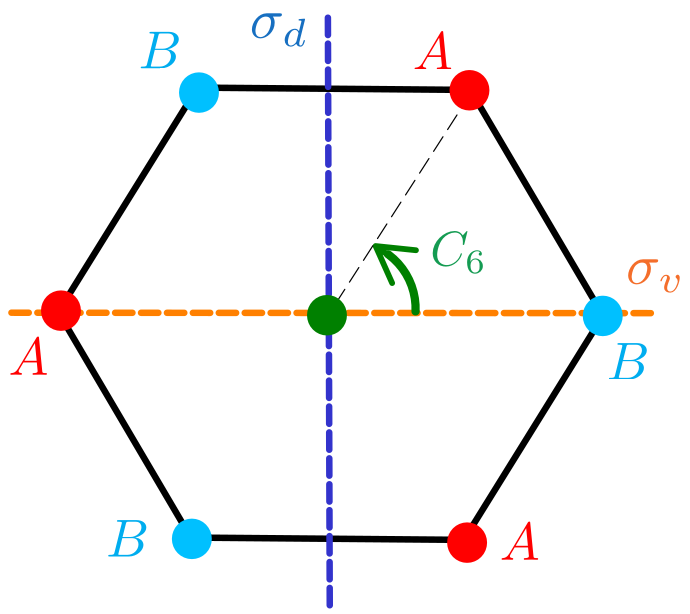
\includegraphics[width=0.4\linewidth]{fig/hexagon_AB.png}
\caption{Symmetries $D_6$ with sublattice type $A$ or $B$.}
\label{fig:hexagon_AB}
\end{figure}

For example, for our generators of $D_6$ we have $\vphi(C_6) = -1$, $\vphi(\sigma_v) = 1$ and $\vphi(\sigma_d) = -1$. Only these values are sufficient, because if we treat $\{1, -1\}$ as a group by itself, with standard multiplication as its operation, one may notice that $\vphi$ follows the rule
$$
\vphi(g_1 g_2) = \vphi(g_1) \vphi(g_2).
$$

The element $g_1 g_2$ changes sublattice only if exactly one of $g_1$ or $g_2$ do. Now, the elements $D_3$ do not exchange sublattice type, which translates to the property $\vphi(g) = 1$ for every $g \in D_3$.

The function $\vphi$ is generally known as a homomorphism, which in the case above identifies the subgroup $D_3$ as its kernel.

\begin{definition}[\textbf{Homomorphism}]
Let $G$ and $H$ be groups. A function $\vphi: G \to H$ is called an \textit{homomorphism} if it preserves the group structure, i.e.,
\begin{equation} \label{eq:homomorphism}
\vphi(a b) = \vphi(a) \vphi(b), \quad \forall \, a,b \in G.
\end{equation}
If $\vphi$ is bijective, we also call it an \textit{isomorphism}. The kernel of $\vphi$ is defined as the set
$$
\ker(\vphi) = \qty{g \in G \mid \vphi(g) = e_H},
$$
where $e_H$ is the identity element of $H$.
\end{definition}

\pagebreak

%%%%%%%%%%%%%%%%%%%%%%%%%%%%%%%%%%%%%%%%%%%%%%%%%%%%%%%%%%%%%%%%%%%%%%%%%%%%%%%%%%%%%%%%%%%%%%%%%%
\section{Elements of Representation Theory}
%%%%%%%%%%%%%%%%%%%%%%%%%%%%%%%%%%%%%%%%%%%%%%%%%%%%%%%%%%%%%%%%%%%%%%%%%%%%%%%%%%%%%%%%%%%%%%%%%%

In physics, specially in Quantum Mechanics, it is most common that one works with groups of matrices, where the theory of Linear Algebra holds. For example, a group of $2\times 2$ matrices isomorphic to $D_6$ can be found by defining the homomorphism $\Phi_2$ below
\begin{equation} \label{eq:D6_generators_2x2matrices}
\Phi_2(\Cs) =
\begin{pmatrix}
\cos(\frac{2\pi}{6}) & \sin(\frac{2\pi}{6}) \\
-\sin(\frac{2\pi}{6}) & \cos(\frac{2\pi}{6})
\end{pmatrix},
\quad
\Phi_2(\sd) =
\begin{pmatrix}
-1 & 0 \\
0 & 1
\end{pmatrix},
\quad
\Phi_2(\sv) =
\begin{pmatrix}
1 & 0 \\
0 & -1
\end{pmatrix}.
\end{equation}

Imposing the homomorphism relation \ref{eq:homomorphism}, we can find all the representative $2\times 2$ matrices of $D_6$ only by multiplying the matrices of the three generators in Equation \ref{eq:D6_generators_2x2matrices}. Because homomorphisms to groups of matrices are so frequent and important, we define:

\begin{definition}[\textbf{Groups of matrices}]
The set of invertible linear operators of a vector space $V$ form a group and we call it the \textit{general linear group}
$$
GL(V) = \qty{A: V \to V \mid A \text{ is linear and invertible}}.
$$
If $V$ is finite dimensional with a scalar product, the set of unitary operators of $V$ is a subgroup of $GL(V)$, defined by
$$
U(V) = \qty{A \in GL(V) \mid A A^\dagger = \1}.
$$
%When $V = \mathbb{R}^n$ or $\C^n$, we can choose a basis and explicitly say that
%$$
%GL(n, \mathbb{R}) = \qty{\text{invertible } n\times n \text{ real matrices}}, \;
%GL(n, \mathbb{C}) = \qty{\text{invertible } n\times n \text{ complex matrices}}.
%$$
%In this case, the subgroups of orthogonal and unitary matrices are, respectively,
%$$
%O(n) = \qty{A \in GL(n, \mathbb{R}) \mid A A^T = \1}, \quad SO(n) = \qty{A \in O(n) \mid \det A = 1};
%$$
%$$
%U(n) = \qty{A \in GL(n, \mathbb{C}) \mid A A^\dagger = \1}, \quad SU(n) = \qty{A \in U(n) \mid \det A = 1}.
%$$
\end{definition}

\begin{definition}[\textbf{Representation}]
A \textit{representation} of a group $G$ on a vector space $V$ is a \textbf{homomorphism} $\Pi: G \to GL(V)$.
\end{definition}

As we learn in Quantum Mechanics (or Linear Algebra), conjugating an operator $H$ by means of $A$, as in $H' = A H A^{-1}$, has the meaning of only changing the reference frame (or the basis). This motivates us to considering two conjugate representations as equivalent:
\begin{definition}[\textbf{Equivalent representations}]
Two representations $\Pi_1: G \to GL(V_1)$ and $\Pi_2: G \to GL(V_2)$ of a group $G$ are said to be \textit{equivalent} if there is an invertible linear operator $A: V_1 \to V_2$ such that
\begin{equation} \label{eq:intertwiner}
\Pi_2(g) = A \Pi_1(g) A^{-1}, \, \forall \, g \in G.
\end{equation}
In this case we write $\Pi_1 \equiv \Pi_2$.
\end{definition}

In Quantum Mechanics, one is usually accostumed to work with unitary matrices and, as we will discuss in the next chapter, there are important orthogonality theorems that hold when we restrict ourselves to unitary representations. This restriction is actually general, as the following theorem asserts \cite{dresselhaus}:
\begin{theorem}[\textbf{Unitarity of representations}] \label{th:unitarity_rep}
Let $V$ be a finite dimensional vector space with a scalar product. A representation $\Gamma: G \to GL(V)$ is called \textit{unitary} if $\Gamma(g) \in U(V)$, $\forall \, g \in G$. Every representation $\Pi: G \to GL(V)$ is equivalent to some unitary representation $\Gamma: G \to U(V)$.
\end{theorem}

Because of Theorem \ref{th:unitarity_rep}, most of our theory will be dedicated to unitary representations. If not otherwise stated, when we say the word ``representation'' we actually mean an \textbf{unitary representation}.

Considering $G = D_3$, take $\Phi_2: G \to GL(V_2)$, $V_2 = \mathbb{R}^2$, as defined in Equation \ref{eq:D6_generators_2x2matrices}, and also consider the trivial representation $\Phi_1: G \to GL(V_1)$, $V_1 = \mathbb{R}$, $\Phi_1(g) = 1$, $\forall \, g \in G$. We can stack $\Phi_2$ and $\Phi_1$ to construct $\Psi: G \to GL(V_0)$, $V_0 = V_2 \oplus V_1$, given by
$$
\Psi(g) =
\begin{pmatrix}
\Phi_2(g) & 0 \\
0 & \Phi_1(g)
\end{pmatrix}, \quad \forall \, g \in G.
$$
\begin{equation} \label{eq:D6_generators_3x3matrices}
\Psi(\Ct) =
\begin{pmatrix}
\cos(\frac{2\pi}{3}) & \sin(\frac{2\pi}{3}) & 0 \\
-\sin(\frac{2\pi}{3}) & \cos(\frac{2\pi}{3}) & 0 \\
0 & 0 & 1
\end{pmatrix},
\;
\Psi(\sd) =
\begin{pmatrix}
-1 & 0 & 0 \\
0 & 1 & 0 \\
0 & 0 & 1
\end{pmatrix},
\;
\Psi(\sv) =
\begin{pmatrix}
1 & 0 & 0 \\
0 & -1 & 0 \\
0 & 0 & 1
\end{pmatrix}.
\end{equation}

We say that the representation $\Psi$ is a direct sum and we write $\Psi \equiv \Phi_2 \oplus \Phi_1$. This is indeed a valid representation, but it kind of does not add much to our knowledge. Representations such as $\Psi$ are called \textit{reducible}. What distinguishes reducible representations are the existence of nontrivial invariant subspaces.
\begin{definition}[\textbf{Invariant subspace}]
A vector subspace $W \subseteq V$ is said to be \textit{invariant} under a representation $\Pi: G \to GL(V)$ if it satisfies $\Pi(g) W \subseteq W$ (the action of $\Pi(g)$ on $W$ is contained within $W$), for every $g \in G$.
\end{definition}

The nontrivial subspaces $V_1$ and $V_2$ are invariant under the action of $\Psi$. Because $\Psi(g)$ is block diagonal for every $g$, we have that $\Psi(g) V_2 \subseteq V_2$ and $\Psi(g) V_1 \subseteq V_1$.
\begin{definition}[\textbf{Irreducible representation}]
A representation $\Pi: G \to GL(V)$ always has the trivial invariant subspace $\{0\}$ and $V$. If there are not others, $\Pi$ is said to be \textit{irreducible}.
\end{definition}

Unlike $\Psi$, the representations $\Phi_1$ and $\Phi_2$ are \textit{irreducible} because they are not equivalent to any representation that is block diagonal. Irreducible representations are building blocks for all representations in finite dimensional vector spaces \cite{dresselhaus}:
\begin{theorem}[\textbf{Decomposition of unitary representations}] \label{th:irreps_decomp}
Let $V$ be a finite dimensional vector space with a scalar product and let $\Gamma: G \to U(V)$ be an unitary representation. Then, $\Gamma$ is either irreducible or reducible and can be decomposed into a direct sum
$$
V = \bigoplus_{j=1}^N V_j, \quad
\Gamma(g) =
\begin{pmatrix}
\pi_1(g) &  &  \\
 & \ddots &  \\
 &  & \pi_N(g) \\
\end{pmatrix},
$$
where each $V_j$ is a nontrivial invariant subspace under $\Gamma$ and $\pi_j: G \to U(V_j)$ is an irreducible representation of $G$.
\end{theorem}

%%%%%%%%%%%%%%%%%%%%%%%%%%%%%%%%%%%%%%%%%%%%%%%%%%%%%%%%%%%%%%%%%%%%%%%%%%%%%%%%%%%%%%%%%%%%%%%%%%
\subsection{Characters}
%%%%%%%%%%%%%%%%%%%%%%%%%%%%%%%%%%%%%%%%%%%%%%%%%%%%%%%%%%%%%%%%%%%%%%%%%%%%%%%%%%%%%%%%%%%%%%%%%%

The trace of a representation is such an important quantity that it deserves the name of its \textit{character}. The \textit{characters} of irreps from a group provides enough information to determine the decomposition of a reducible representation into irreducible ones, as in Theorem \ref{th:irreps_decomp}.

\begin{definition}[\textbf{Character}]
The \textit{character} of an element $g \in G$ in the representation $\Pi: G \to GL(V)$ is defined as
\begin{equation} \label{eq:character}
\chi(g) = \tr[\Pi(g)] = \sum_{j} \Pi_{jj}(g).
\end{equation}
\end{definition}
Due to the cyclic property of the trace of a matrix, equivalent irreducible representations (irreps) have the same characters
$$
\chi'(g) = \tr[A^{-1} \Pi(g) A] =  \tr[AA^{-1} \Pi(g)] = \chi(g).
$$
Also, elements from the same conjugacy class $g$ and $g' = a g a^{-1}$ also have the same character
$$
\chi(g') = \chi(aga^{-1}) = \tr[\Pi(aga^{-1})] = \tr[\Pi(a)\Pi(g)\Pi(a^{-1})] = \tr[\Pi(a^{-1})\Pi(a)\Pi(g)] = \chi(g).
$$

Due to this fact, one could also speak of the character of a conjugacy class $S = [g]$, where we denote it by $\chi_S = \chi(g) = \chi(g')$.

Now we are going to state some theorems about characters, which are known as ``Wonderful Orthogonality Theorems'' \cite{dresselhaus, hamermesh}.

\begin{theorem}[\textbf{1st Wonderful Orthogonality Theorem}] \label{th:1st-wot}
The characters $\chi^{(\Gamma_i)}$, $\chi^{(\Gamma_j)}$ of irreducible representations $\Gamma_i, \Gamma_j: G \to U(V)$ obey the orthogonality relation
\begin{equation} \label{eq:1st-wot}
\delta_{\Gamma_i, \Gamma_j} =
\frac{1}{\abs{G}} \sum_{g \in G} \chi^{(\Gamma_i)}(g) \chi^{(\Gamma_j)}(g)^* =
\frac{1}{\abs{G}} \sum_{S} \abs{S} \, \chi^{(\Gamma_i)}_S \qty[\chi^{(\Gamma_j)}_S]^*,
\end{equation}
where the sum in $S$ runs through the conjugacy classes of $G$, with $\abs{S}$ denoting the number of elements of the class $S$.
\end{theorem}

If we consider a $n_{\text{classes}} -$dimensional vector space, with the vectors with a fixed irreps $\Gamma_i$
$$
\ket{\psi^{(\Gamma_i)}} =
\qty(
\sqrt{\frac{\abs{S_1}}{\abs{G}}} \chi^{(\Gamma_i)}_{S_1},
\sqrt{\frac{\abs{S_2}}{\abs{G}}} \chi^{(\Gamma_i)}_{S_2},
\ldots,
\sqrt{\frac{\abs{S_m}}{\abs{G}}} \chi^{(\Gamma_i)}_{S_{n_{\text{classes}}}}
),
$$
where $n_{\text{classes}}$ is the number of different classes of $G$, then Theorem \ref{th:1st-wot} can be in fact viewed as an orthogonality relation because we can rewrite Equation \ref{eq:1st-wot} as
\begin{equation} \label{eq:orthog_irreps}
\braket{\psi^{(\Gamma_i)}}{\psi^{(\Gamma_j)}} = \delta_{\Gamma_i, \Gamma_j}.
\end{equation}

A consequence of this orthogonality relation is that there are no more than $n_{\text{classes}}$ of such vectors. If there were more, they would be linearly dependent, contradicting Equation \ref{eq:orthog_irreps}. From this, the number of irreps satisfies $n_{\text{irreps}} \leq n_{\text{classes}}$.

\begin{theorem}[\textbf{2nd Wonderful Orthogonality Theorem}] \label{th:2nd-wot}
Let $\Gamma_j: G \to U(V)$ be the irreducible representations of $G$. The summation over all irreps
\begin{equation} \label{eq:2nd-wot}
\frac{1}{\abs{G}} \sum_{\Gamma_j} \abs{S} \, \chi^{(\Gamma_j)}_S \qty[\chi^{(\Gamma_j)}_{S'}]^* = \delta_{S, S'}
\end{equation}
also yields an orthogonality relation, where $S$ and $S'$ are conjugacy classes of $G$.
\end{theorem}

\begin{corollary} \label{coro:chi_E}
Applying Theorem \ref{th:2nd-wot} to the trivial class $S = S' = \{E\}$, we obtain
\begin{equation} \label{eq:chi_E_coro}
\abs{G} = \sum_{\Gamma_j} \abs{\chi^{(\Gamma_j)}(E)}^2 = \sum_{\Gamma_j} \ell_j^2,
\end{equation}
where $\ell_j = \chi^{(\Gamma_j)}(E)$ is the dimension of the irrep $\Gamma_j$.
\end{corollary}

Now we can apply the same reasoning considering a $n_{\text{irreps}}-$dimensional vector space with the vectors for a fixed class $S$
$$
\ket{\phi_{S}} =
\qty(
\sqrt{\frac{\abs{S}}{\abs{G}}} \chi^{(\Gamma_1)}_{S},
\sqrt{\frac{\abs{S}}{\abs{G}}} \chi^{(\Gamma_2)}_{S},
\ldots,
\sqrt{\frac{\abs{S}}{\abs{G}}} \chi^{\qty(\Gamma_{n_{\text{irreps}}})}_{S}
),
$$

Analogously, Theorem \ref{th:2nd-wot} implies the orthogonality
$$
\braket{\phi_{S}}{\phi_{S'}} = \delta_{S, S'}.
$$

As such, we also conclude that $n_{\text{classes}} \leq n_{\text{irreps}}$. Now we can announce the theorem:

\begin{theorem}[$\bm{n_{\textbf{irreps}} = n_{\textbf{classes}}}$] \label{th:num_irreps_classes}
The number of irreducible representations of a group $G$ is equal to its number of conjugacy classes.
\end{theorem}

With theorems \ref{th:1st-wot}, \ref{th:2nd-wot} and \ref{th:num_irreps_classes} we can construct the \textbf{TABLE OF CHARACTERS}. Let us come back to the $G = D_3$ example. We already established two irreducible representations $\Phi_1$ and $\Phi_2$. As we know from Equation \ref{eq:D3_classes}, the group $D_3$ has three distinct classes, thus also three inequivalent irreducible representations. Calculating the characters of the classes from Equation \ref{eq:D3_classes} under $\Phi_1$ and $\Phi_2$, we obtain
$$
\chi^{(\Phi_1)}(E) = \chi^{(\Phi_1)}(\Ct) = \chi^{(\Phi_1)}(\sv) = 1
$$
$$
\chi^{(\Phi_2)}(E) = 2, \quad \chi^{(\Phi_2)}(\Ct) = 2 \cos(\frac{2\pi}{3}) = -1, \quad \chi^{(\Phi_2)}(\sv) = 0.
$$

Applying Theorem \ref{th:2nd-wot} with $S = S' = \{E\}$, the trivial conjugacy class with only the identity element, we obtain the relation
\begin{equation} \label{eq:chi_E}
\abs{G} = \sum_{\Gamma_j} \abs{\chi^{(\Gamma_j)}(E)}^2 = \sum_{\Gamma_j} \ell_j^2,
\end{equation}
where $\chi^{(\Gamma_j)}(E) = \ell_j$ is the dimensionality of the representation $\Gamma_j$. Using Equation \ref{eq:chi_E} with $G = D_3$, we obtain
$$
6 = 2^2 + 1^2 + \ell_3^2 \implies \ell_3 = 1,
$$
which tells us that the last irrep $\Gamma_3$ is an one-dimensional representation. Because of this, the matrix representatives are numbers, and $\Gamma_3(g) = \chi^{(\Gamma_3)}(g)$. Using that $C_3^3 = E$, we have $\Gamma_3(C_3)^3 = 1$, which implies that $\Gamma_3(C_3) = 1$. Analogously, $\sigma_v^2 = E \implies \Gamma_3(\sigma_v)^2 = 1$. But notice that, if $\Gamma_3$ would be $1$, we would end up with $\Gamma_3 \equiv \Gamma_1$. Therefore, the correct solution is $\Gamma_3(\sigma_v) = -1$. Summing up, we have
$$
\chi^{(\Gamma_3)}(E) = 1, \quad \chi^{(\Gamma_3)}(\Ct) = 1, \quad \chi^{(\Gamma_3)}(\sv) = -1.
$$

With all irreps, classes and characters known, we can now construct the table of characters for the group $D_3$:
\begin{table}[H]
\caption{Character table of group $D_3$.}
\centering
\begin{tabular} { c c c c }
\specialrule{0.05em}{0em}{0.2em}
$\P$ & $\P E$ & $\P 2 C_3$ & $\P 3 C_2'$ \\
\specialrule{0.01em}{0.2em}{0.2em}
$A_1$ & $\P1$ & $\P1$ & $\P1$ \\
\specialrule{0.01em}{0.2em}{0.2em}
$A_2$ & $\P1$ & $\P1$ & $ -1$ \\
\specialrule{0.01em}{0.2em}{0.2em}
$E$   & $\P2$ & $ -1$ & $\P0$ \\
\specialrule{0.05em}{0.2em}{0em}
\end{tabular}
\label{tab:D3}
\end{table}

The same procedure could be applied to construct the table for the group $D_3$, which we show in Table \ref{tab:D6}.
\begin{table}[H]
\caption{Character table of point group $D_6$.}
\centering
\begin{tabular} { c c c c c c c  }
\specialrule{0.05em}{0em}{0.2em}
$\P$ & $\P E$ & $\P C_2$ & $\P2C_3$ & $\P2C_6$ & $\P3C_2'$ & $\P3C_2''$ \\
\specialrule{0.01em}{0.2em}{0.2em}
$A_1$ & $\P1$ & $\P1$ & $\P1$ & $\P1$ & $\P1$ & $\P1$ \\
\specialrule{0.01em}{0.2em}{0.2em}
$A_2$ & $\P1$ & $\P1$ & $\P1$ & $\P1$ & $ -1$ & $ -1$ \\
\specialrule{0.01em}{0.2em}{0.2em}
$B_1$ & $\P1$ & $ -1$ & $\P1$ & $ -1$ & $\P1$ & $ -1$ \\
\specialrule{0.01em}{0.2em}{0.2em}
$B_2$ & $\P1$ & $ -1$ & $\P1$ & $ -1$ & $ -1$ & $\P1$ \\
\specialrule{0.01em}{0.2em}{0.2em}
$E_1$ & $\P2$ & $ -2$ & $ -1$ & $\P1$ & $\P0$ & $\P0$ \\
\specialrule{0.01em}{0.2em}{0.2em}
$E_1$ & $\P2$ & $\P2$ & $ -1$ & $ -1$ & $\P0$ & $\P0$ \\
\specialrule{0.05em}{0.2em}{0em}
\end{tabular}
\label{tab:D6}
\end{table}

\begin{theorem}[\textbf{Reduction formula}] \label{th:reduction_formula}
By Theorem \ref{th:irreps_decomp}, a representation $\Gamma: G \to U(V)$ is a direct sum of irreps
$$
\Gamma \equiv \bigoplus_j r_j \, \Gamma_j,
$$
where the coefficients $r_j \in \N_{>0}$ denote the number of times the irrep $\Gamma_j$ appears in the decomposition of $\Gamma$. The coefficients $r_j$ are given by the \textit{reduction formula}
\begin{equation} \label{eq:reduction_formula}
r_j =
\frac{1}{\abs{G}} \sum_{g \in G} \chi^{(\Gamma)}(g) \chi^{(\Gamma_j)}(g)^* =
\frac{1}{\abs{G}} \sum_{S} \abs{S} \, \chi^{(\Gamma)}_S \qty[\chi^{(\Gamma_j)}_S]^*.
\end{equation}
\end{theorem}

Utilize it with conjuction with the reduction formula \ref{th:reduction_formula} to determine the decomposition of whichever representation of a group.

\begin{example}
teste
\end{example}

<++>

%%%%%%%%%%%%%%%%%%%%%%%%%%%%%%%%%%%%%%%%%%%%%%%%%%%%%%%%%%%%%%%%%%%%%%%%%%%%%%%%%%%%%%%%%%%%%%%%%%
\subsection{Induction and subduction of representations}
%%%%%%%%%%%%%%%%%%%%%%%%%%%%%%%%%%%%%%%%%%%%%%%%%%%%%%%%%%%%%%%%%%%%%%%%%%%%%%%%%%%%%%%%%%%%%%%%%%

Let us consider an irreducible representation $\Gamma$ of a group $G$. Now, given a subgroup $H$ of $G$, we can construct the so-called \textit{subduced} representation of $H$, formed by the matrices of those elements of $G$ that also belong to $H$, that is $\Gamma(h)$ for $h \in H$. This representation is in general reducible, and it is denoted by $\Gamma \downarrow H$.

Thinking in the other direction, if we start with an irreducible representation $D$ of $H \leq G$, we can construct the so-called \textit{induced} representation of $D \uparrow G = \Delta$ of $G$, as follows
\begin{align*}
\Delta_{i'j'ij}(g) =
\begin{cases}
\; D_{i'i}(g_{j'}^{-1} g g_j), \quad & g_{j'}^{-1} g g_j \in H, \\
\; 0,  & g_{j'}^{-1} g g_j \notin H.
\end{cases}
\end{align*}


%%%%%%%%%%%%%%%%%%%%%%%%%%%%%%%%%%%%%%%%%%%%%%%%%%%%%%%%%%%%%%%%%%%%%%%%%%%%%%%%%%%%%%%%%%%%%%%%%%
\section{Space Groups}
%%%%%%%%%%%%%%%%%%%%%%%%%%%%%%%%%%%%%%%%%%%%%%%%%%%%%%%%%%%%%%%%%%%%%%%%%%%%%%%%%%%%%%%%%%%%%%%%%%


Essentially, when working with group theory in the context of solids, we are interested in subgroups of a particular group of matrices. These are called orthogonal matrices, and are defined by $R R^T = E$, where $E$ here is the identity matrix.

\n

The point group and translation symmetry operations which carry the crystal into itself form a group called the \textit{space group}. The elements of it are commonly denoted by  $\{ R_\alpha \mid \tau \} $, where $R_\alpha$ is the point group operation and $\tau$ is the translation.

Pure rotations and pure translations are special cases of space group operations:
\begin{itemize}
\item $\sg{\eps}{0} =$ identity.
\item $\sg{R_\alpha}{0} =$ pure point group operation.
\item $\sg{\eps}{\tau} =$ pure translation.
\end{itemize}

The result for the multiplication of two space group operations is
$$
\sg{R_\beta}{\tau_2} \sg{R_\alpha}{\tau_1} = \sg{R_\beta R_\alpha}{R_\beta\tau_1 + \tau_2}.
$$

Beyond pure operations, we may find compound operations that combine translations and point group operations. The two possible types are \textit{glide planes} and \textit{screw axes}.
\begin{figure}[H]
\centering
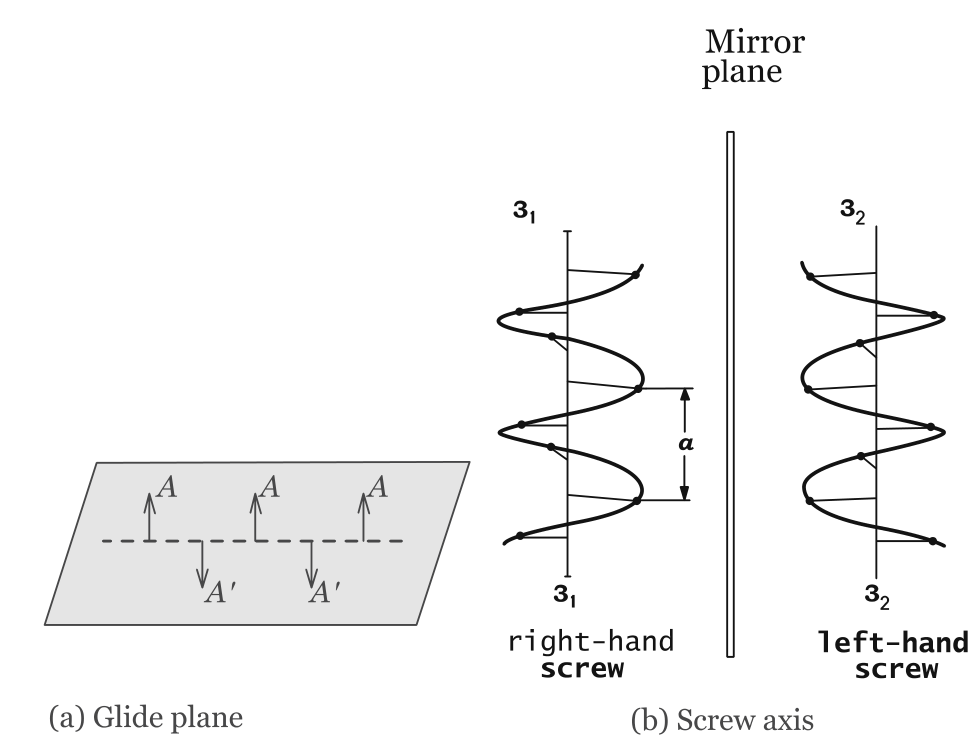
\includegraphics[width=0.5\linewidth]{fig/glideplane-screwaxis.png}
\caption{(a) The glide plane takes $A$ into $A'$. (b) Right- and left-hand screw axis.}
\label{fig:glideplane-screwaxis}
\end{figure}

Here we are going to study the concept of \textit{space groups}. It is very important to classify the symmetry properties of the system in interest (Twisted Bilayer Graphene). In our examples, we are going to focus on the familiar honeycomb lattice example. The space group is loosely an semi-direct product of the point group and the translation group. Given a fixed lattice, all the linear transformations that carry the lattice into itself belong to the space group. A useful matrix representation for $G$ is:
\begin{equation} \label{eq:spacegroup-rep}
\sg{R_\alpha}{\vtau} =
\begin{pmatrix}
1 & 0 \\
\vtau & R_\alpha
\end{pmatrix},
\end{equation}
where $0$ is a row of three zeros, $\vtau$ is a column vector and $R_\alpha$ is $3\times 3$ rotation matrix.

The inverse of an element is given by
\begin{equation} \label{eq:inv-spacegroup}
\sg{R_\alpha}{\vtau}^{-1} =
\begin{pmatrix}
1 & 0 \\
-R_\alpha^{-1}\vtau & R_\alpha^{-1}
\end{pmatrix} =
\sg{R_\alpha^{-1}}{-R_\alpha^{-1}\vtau}.
\end{equation}

Let's take the honeycomb lattice as the example. The space group of interest $P622$ \cite{thesis_rennella} is symmorphic (Table 9.1 of \cite{dresselhaus}). Therefore it is impossible to find a screw axis or glide plane. We have to rely on pure translation + pure point group.

\textbf{IT IS MUCH BETTER TO MAKE THE EXAMPLE 2x2}

For example, let's take a translation of $d(\cos30^\circ, \sin30^\circ)$ with a rotation of $60^\circ$. The result is
$$
R_{\mathcal{E}} =
\begin{pmatrix}
\frac{1}{2} & -\frac{\sqrt{3}}{2} \\
\frac{\sqrt{3}}{2} & \frac{1}{2} \\
\end{pmatrix}
$$

Consider the two basis $\mathcal{E} = \{\ihat, \jhat\}$, and $\mathcal{B} = \{\v_1, \v_2\}$, where $\v_1 = a \ihat$, and $\v_2 = a \qty(\frac{1}{2}\ihat + \frac{\sqrt{3}}{2} \jhat)$. The change of basis matrix is from $\mathcal{B}$ to $\mathcal{E}$ is $M_{\mathcal{B}\to\mathcal{E}}$ and its inverse is $M_{\mathcal{E}\to\mathcal{B}} = M_{\mathcal{B}\to\mathcal{E}}^{-1}$
$$
M_{\mathcal{B} \to \mathcal{E}} =
a
\begin{pmatrix}
1 & \frac{1}{2} \\
0 & \frac{\sqrt{3}}{2}
\end{pmatrix},
\quad
M_{\mathcal{E} \to \mathcal{B}} = M_{\mathcal{B}\to\mathcal{E}}^{-1} =
\frac{1}{a}
\begin{pmatrix}
1 & -\frac{1}{\sqrt{3}} \\
0 & \frac{2}{\sqrt{3}}
\end{pmatrix},
$$

In this basis, the rotation matrix becomes
$$
R_{\mathcal{B}} =  M_{\mathcal{E} \to \mathcal{B}} \, R_{\mathcal{E}} \, M_{\mathcal{B}\to\mathcal{E}} =
\begin{pmatrix}
0 & -1 \\
1 &  0
\end{pmatrix}
$$

The translation of $d(\cos 30^\circ, \sin 30^\circ)$ is
$$
\bm{\tau}_E = a \begin{pmatrix} \frac{1}{2} \\ \frac{\sqrt{3}}{6} \end{pmatrix} \implies
\bm{\tau}_B = M_{\mathcal{E} \to \mathcal{B}} \bm{\tau}_E =
\begin{pmatrix}
\frac{1}{3} \\ \frac{1}{3}
\end{pmatrix}.
$$

Our space group matrix (in the $\mathcal{B}$ basis) is
$$
\{R_{\mathcal{B}}, \vtau_{\mathcal{B}}\} =
\begin{pmatrix}
1 & 0 & 0 \\
1/3 & 0 & -1 \\
1/3 & 1 & 0 \\
\end{pmatrix}
$$

Some arbitrary lattice vector is represented by $\u_s = m \v_1 + n\v_2 + \bm{\beta_s}$, where $s = A, B$ represents the sublattice index, with $\bm{\beta}_A = \0$, $\bm{\beta}_B = \vtau_{\mathcal{B}}$. We have
$$
\{R_{\mathcal{B}}, \vtau_{\mathcal{B}}\} \, \u_A =
\begin{pmatrix}
1 & 0 & 0 \\
1/3 & 0 & -1 \\
1/3 & 1 & 0 \\
\end{pmatrix}
\begin{pmatrix}
1 \\ m \\ n
\end{pmatrix}
=
$$
$$
=
\begin{pmatrix}
1 \\ -n + \frac{1}{3} \\ m+n+\frac{1}{3}
\end{pmatrix}
=
\begin{pmatrix}
1 \\ -n \v_1 + (m+n) \v_2 + \vtau_{\mathcal{B}}
\end{pmatrix}
\in B.
$$

$$
\{R_{\mathcal{B}}, \vtau_{\mathcal{B}}\} \, \u_B =
\begin{pmatrix}
1 & 0 & 0 \\
1/3 & 0 & -1 \\
1/3 & 1 & 0 \\
\end{pmatrix}
\begin{pmatrix}
1 \\ m + \frac{1}{3} \\ n + \frac{1}{3}
\end{pmatrix}
=
$$
$$
=
\begin{pmatrix}
1 \\ -n \\ 1+m+n
\end{pmatrix}
=
\begin{pmatrix}
1 \\ -n \v_1 + (1+m+n) \v_2
\end{pmatrix}
\in A.
$$

Therefore, the lattice is invariant by the space group operation $\{R_{\mathcal{B}}, \vtau_{\mathcal{B}}\}$.

\n

\textbf{Example of nonsymmorphic space group}: Tellurium screw axis $3_1$ (achei figura na internet). Glide plane triangular lattice (gerar minha própria figura), translation $a/2$ and reflection. There is also this link \href{https://physics.stackexchange.com/questions/568476/example-of-a-space-group-which-does-not-contain-the-point-group-as-a-subgroup}{here} which explains the glide plane symmetry in Kagomé lattice. \textbf{Maybe it is better to consider the H2O ice hexagonal.}

%\section{Site-symmetry group}
%
%Let $G$ be a space group associated with its corresponding lattice and a choice of origin. The subgroup of all symmetry operations of $G$ that leaves a point $P$ of the real space inveriant is called the \textit{site-symmetry group} of $P$. This point $P$ is called \textit{of special position} with respect to $G$ if there is at least one non-trivial (not the identity) symmetry operation of $G$ that leaves $P$ invariant.
%
%For a general operation $g$ of $G$, the point $P$ will be mapped into some other point $Q = g P$. If $P$ is of special position with site-symmetry group $G_P$, then $Q$ will also be of special position and its site-symmetry group $G_Q$ will be a conjugate group of $G_P$, namely $G_Q = g G_P g^{-1}$. In fact, we have
%$$
%G_Q Q = g G_P g^{-1} Q = g G_P P = g P = Q.
%$$
%
%If we apply of all operations of $G$ to $P$, we obtain the \textit{crystallographic orbit} of $P$, which is the set of points $Q$ with site-symmetry groups conjugate to $G_P$. If $P$ is of special position, we call its crystallographic orbit a \textit{Wyckoff position} of the space group $G$. Therefore, the concept of Wyckoff position refers to a \textbf{set of points of special position with site-symmetry groups conjugates of each other}.

%%%%%%%%%%%%%%%%%%%%%%%%%%%%%%%%%%%%%%%%%%%%%%%%%%%%%%%%%%%%%%%%%%%%%%%%%%%%%%%%%%%%%%%%%%%%%%%%%%
\subsection{Translation subgroup}
%%%%%%%%%%%%%%%%%%%%%%%%%%%%%%%%%%%%%%%%%%%%%%%%%%%%%%%%%%%%%%%%%%%%%%%%%%%%%%%%%%%%%%%%%%%%%%%%%%

All the elements $\sg{\eps}{\tau}$ of the the space group $G$ constitute the translation group $T$. It is a subgroup of $G$ and defines the Bravais lattice. More than that, $T$ is a normal subgroup of $G$, which means that $g T g^{-1} = T$ for every $g \in G$. Because of that, the cosets
$$
\{ \sg{R_\alpha}{\tau'} \sg{\eps}{\tau} \mid \sg{\eps}{\tau} \in T \} \in G/T
$$
form a factor group of the space group $G$.

This factor group $G/T$ is actually isomorphic to the point group of $G$.

%%%%%%%%%%%%%%%%%%%%%%%%%%%%%%%%%%%%%%%%%%%%%%%%%%%%%%%%%%%%%%%%%%%%%%%%%%%%%%%%%%%%%%%%%%%%%%%%%%
\subsection{Symmorphic and Nonsymmorphic Space Groups}
%%%%%%%%%%%%%%%%%%%%%%%%%%%%%%%%%%%%%%%%%%%%%%%%%%%%%%%%%%%%%%%%%%%%%%%%%%%%%%%%%%%%%%%%%%%%%%%%%%

In a space group $G$, we can always rewrite its elements in the form
$$
\sg{R_\alpha}{\tau} = \sg{R_\alpha}{r_n + \tau} = \sg{\eps}{r_n} \sg{R_\alpha}{\tau_\alpha},
$$
where $r_n$ is a general vector of the Bravais lattice and $\tau_\alpha$ is either zero or a non-primitive Bravais lattice translation. Basically, we will have $\tau_\alpha = 0$ for simple group operations and $\tau_\alpha \neq 0$ for glide planes or screw axis.

If, with a suitable choice of origin, all the elements of $G$ can be written in the form $\sg{R_\alpha}{\tau} = \sg{R_\alpha}{r_n} = \sg{\eps}{r_n} \sg{R_\alpha}{0}$ ($\tau_\alpha = 0$ for every symmetry operation), then call $G$ a \textit{symmorphic} space group.


%%%%%%%%%%%%%%%%%%%%%%%%%%%%%%%%%%%%%%%%%%%%%%%%%%%%%%%%%%%%%%%%%%%%%%%%%%%%%%%%%%%%%%%%%%%%%%%%%%%
%\section{Space groups in Reciprocal Space}
%%%%%%%%%%%%%%%%%%%%%%%%%%%%%%%%%%%%%%%%%%%%%%%%%%%%%%%%%%%%%%%%%%%%%%%%%%%%%%%%%%%%%%%%%%%%%%%%%%%
%
%%%%%%%%%%%%%%%%%%%%%%%%%%%%%%%%%%%%%%%%%%%%%%%%%%%%%%%%%%%%%%%%%%%%%%%%%%%%%%%%%%%%%%%%%%%%%%%%%%%
%\subsection{Group of the wave vector $G_{\k}$ and the Star of $\k$}
%%%%%%%%%%%%%%%%%%%%%%%%%%%%%%%%%%%%%%%%%%%%%%%%%%%%%%%%%%%%%%%%%%%%%%%%%%%%%%%%%%%%%%%%%%%%%%%%%%%
%
%If we have
%$$
%(\hat{P}_\alpha \R_n) \vdot \K_m = 2 \pi N,
%$$
%than
%$$
%\R_n \vdot (\hat{P}_\alpha^{-1} \K_m) = 2 \pi N.
%$$
%
%Thus, the effect of an operator $\hat{P}_\alpha$ on a direct lattice vector $\R_n$ is equivalent to the effect of the operator $\hat{P}_\alpha^{-1}$ on the corresponding reciprocal lattice vector $\K_m$.
%
%\n
%
%The group of the wave vector is formed by the set of space group operations which transform $\k$ into itself, or into an equivalent $\k = \k + \K_m$, where $\K_m$ is a vector of the reciprocal lattice.
%
%All the symmetry operation of the space group $G$ take the point $\k = 0$ into an equivalent point, so that the group of the wave vector at $\k = 0$ corresponds to $G$. Furthermore, the $G_\k$ for $\k \neq 0$ remains a subgroup of $G$.
%
%\n
%
%The set of wave vectors $\k'$ which are obtained by carrying out all the point group operations on $\k$ is called \textit{star of} $\k$.
%
%\n
%
%In summary
%$$
%\text{real space} \iff \text{reciprocal space}
%$$
%$$
%\text{site-symmetry group} \iff \text{group of wave vector }G_\k
%$$
%$$
%\text{Wyckoff position} \iff \text{star of }\k
%$$

\section{Magnetic Space Groups}

Magnetic moments in a solid appears when there are unpaired electrons in electronic shells. A common example is the Hund's rule, which favours the ``ferromagnetic'' interaction so that an intrinsic magnetic moment appears. Below the ordering temperature, a magnetic structure is formed, and above the ordering temperature, the system is in the paramagnetic state.

In this section, we are going to introduce the concept of magnetic space group (Shubnikov group), which is important to study magnetic structures. But our main interest is to apply its theory to analyze symmetries of the TBG system, which has negligible SOC and we can say ``it is spinless'', but we can use the same formalism on the sublattice degree of freedom.

To study the symmetries of magnetic configurations, we introduce the time reversal operator, denoted by $T$ or $1'$. In the context of magnetic systems, this operator acts on magnetic moments that are ``classical axial vectors''. Its action consists of reverting the sense of the current loop, so that the orientation of the magnetic moment is reversed.

\begin{figure}[H]
\centering
\begin{subfigure}{.4\textwidth}
  \centering
  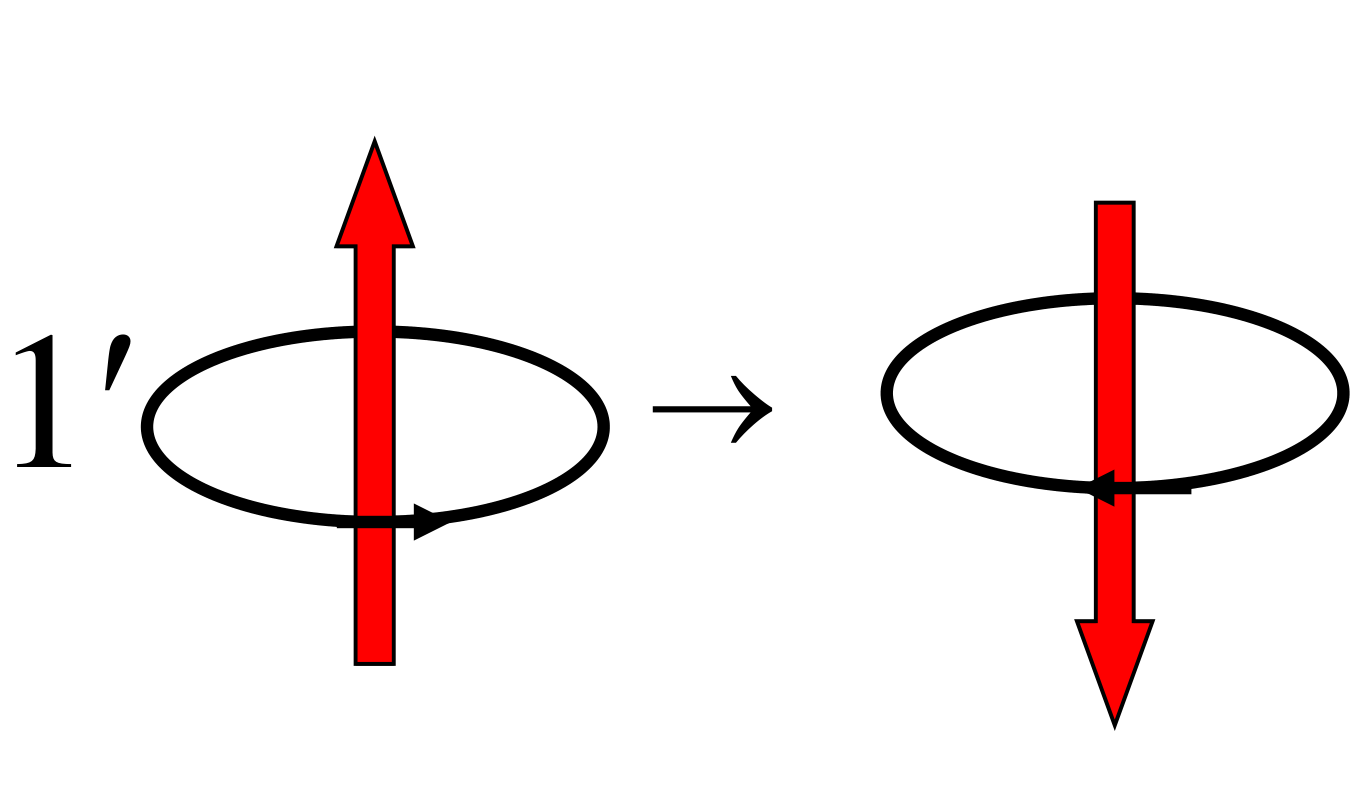
\includegraphics[height=0.4\linewidth]{fig/timerev.png}
  \caption{}
  \label{fig:timerev}
\end{subfigure}%
\begin{subfigure}{.6\textwidth}
  \centering
  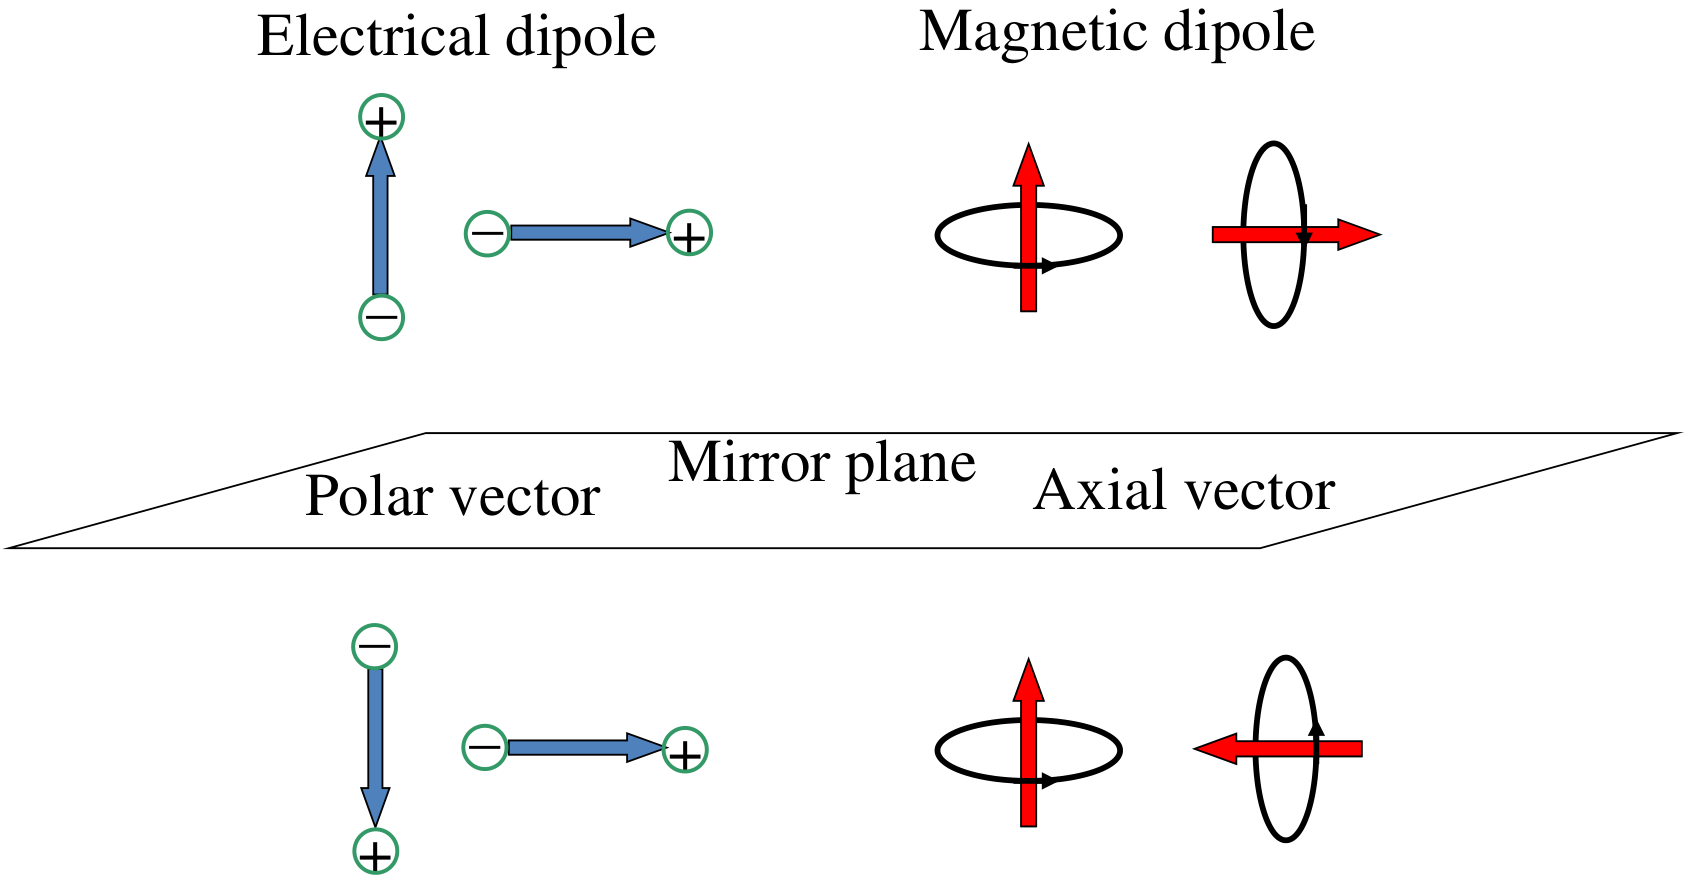
\includegraphics[width=\linewidth]{fig/axialvec.png}
  \caption{}
  \label{fig:axialvec}
\end{subfigure}
\caption{.}
\label{fig:geometry}
\end{figure}

We define the time reversal group formed by only two elements $R = \{1, 1'\}$. Any magnetic group $M$ can be obtained as a subgroup of the direct product of $R$ with another group $G$, such that $M \leq G \otimes R$. The group $G \otimes \{1\}$ is a magnetic group, called ``colourless''. The paramagnetic (``grey'') groups are of the form $P = G \cup G1'$. The other form to construct magnetic groups (``black-white'') is
$$
M = H + (G - H) 1',
$$
where $H \leq G$ is a subgroup of index 2.


\section{Application to TBG}

The magnetic point group of the BM model of TBG is $6'2'2$ in Hermann-Mauguin notation. According to the notation, we can choose its generators to be $C_{6z} T$, $C_{2y} T$ and $C_{2x}$.

\begin{figure}[H]
\centering
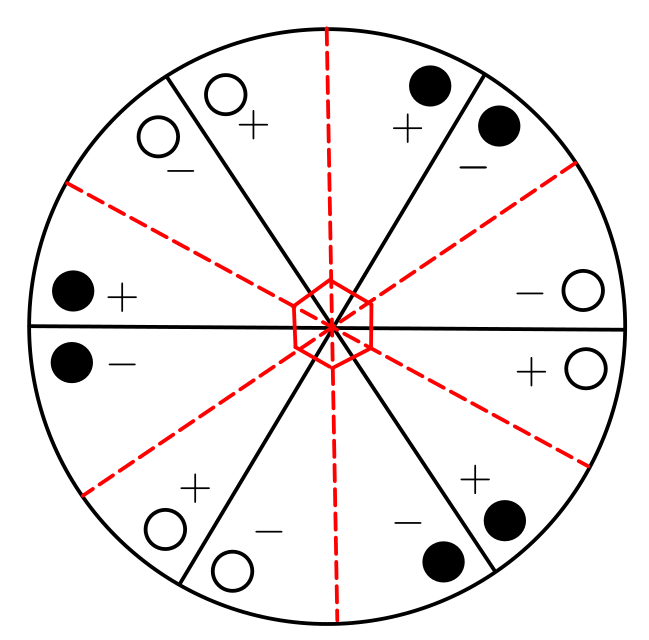
\includegraphics[width=0.5\linewidth]{fig/622_magnetic.png}
\caption{Representation of the magnetic point group $6'2'2$.}
\label{fig:622_magnetic}
\end{figure}





%%%%%%%%%%%%%%%%%%%%%%%%%%%%%%%%%%%%%%%%%%%%%%%%%%%%%%%%%%%%%%%%%%%%%%%%%%%%%%%%%%%%%%%%%%%%%%%%%%
%%%%%%%%%%%%%%%%%%%%%%%%%%%%%%%%%%%%%%%%%%%%%%%%%%%%%%%%%%%%%%%%%%%%%%%%%%%%%%%%%%%%%%%%%%%%%%%%%%


%%%%%%%%%%%%%%%%%%%%%%%%%%%%%%%% COMMENT THIS TO COMPILE main.tex %%%%%%%%%%%%%%%%%%%%%%%%%%%%%%%%
%%-----
%% Referências bibliográficas
%%-----
\addcontentsline{toc}{chapter}{\bibname}
%\bibliographystyle{abntex2-num}
\bibliography{citations}
\bibliographystyle{ieeetr}
\end{document}
%%%%%%%%%%%%%%%%%%%%%%%%%%%%%%%% COMMENT THIS TO COMPILE main.tex %%%%%%%%%%%%%%%%%%%%%%%%%%%%%%%%
